\section{Weak Lensing}\label{sec:wl}

The LSST provides an opportunity to mitigate WL systematics using the observing strategy. This opportunity was not possible in previous surveys because the LSST will be the first survey to dither at large scales (relative to the field of view) with a large number of exposures.

We analyzed how different OpSim runs perform with respect to the point-spread function (PSF) modeling errors and similar WL systematics as follows: (a) We create 50 million stars uniformly in the WFD areas of each survey, with cuts based on the coadded depth and dust extinction, consistently the LSS WG. (b) we model the PSF modeling errors at each star in each exposure as a 6\% radial error in the outer 20\% of field of view (and no error). We assume an average size error on the PSF model of . This model is realistically motivated by recent surveys (e.g. \cite{bosche2018}) (c) We average down the modeling errors across exposures via their second moments, where this operation is linear. You can read more about this process on GitHub \footnote{\url{https://github.com/hsnee/lsstpsf/blob/master/methodology.ipynb}} (d) Propagate the averaged errors into bias on the cosmic shear using the $\rho$-statistics formulation (\cite{rowe2010}; \cite{jarvis2016}). The code to recreate this analysis is available on GitHub \footnote{\url{https://github.com/hsnee/lsstpsf/blob/master/ModelErrorsNew.ipynb}}. 

Figure~\ref{fig:WLSystematicsRankings} shows the result of this analysis, propagated into bias on the cosmic shear signal. 

Table~\ref{table:WLSystematicsRankings} provides a ranking of the strategies. There are certain trends that can be seen from the table (or equivalently, from figure~\ref{fig:WLSystematicsRanking}): more visits in the main WFD survey are very useful for averaging down weak lensing systematics (whether achieved by smaller area, or shorter 20 second visits.) OpSim runs with more exposure to the galactic planes underperform. Runs with rolling cadence significantly underperform others, especially ones that have rolling cadence in all or most years. These are not surprising trends, since prioritizing uniformity in WFD over area increases and rolling strategies is what would essentially drive weak lensing systematics down. Table~\ref{table:WLSystematicsRankings} also shows the average number of exposures in $i$-band for 5000 objects randomly drawn from a uniform distribution throughout the areas covered by each of the OpSim runs, and shows a strong correlation between this number and the performance of the runs. Rolling cadence runs and wider area runs also appear to have significant number of average visits. We are also exploring additional explanations of why rolling cadence runs are consistently underperforming.


\begin{figure}[htb]
    \centering
    \caption{The bias on the cosmic shear signal as a function of angular separation for all recent OpSim runs, at years 1, 3, 6, and 10. This indicates their performance with respect to weak lensing systematics, with higher curves corresponding to higher bias/worse performance.}
    \label{fig:WLSystematicsRankings}
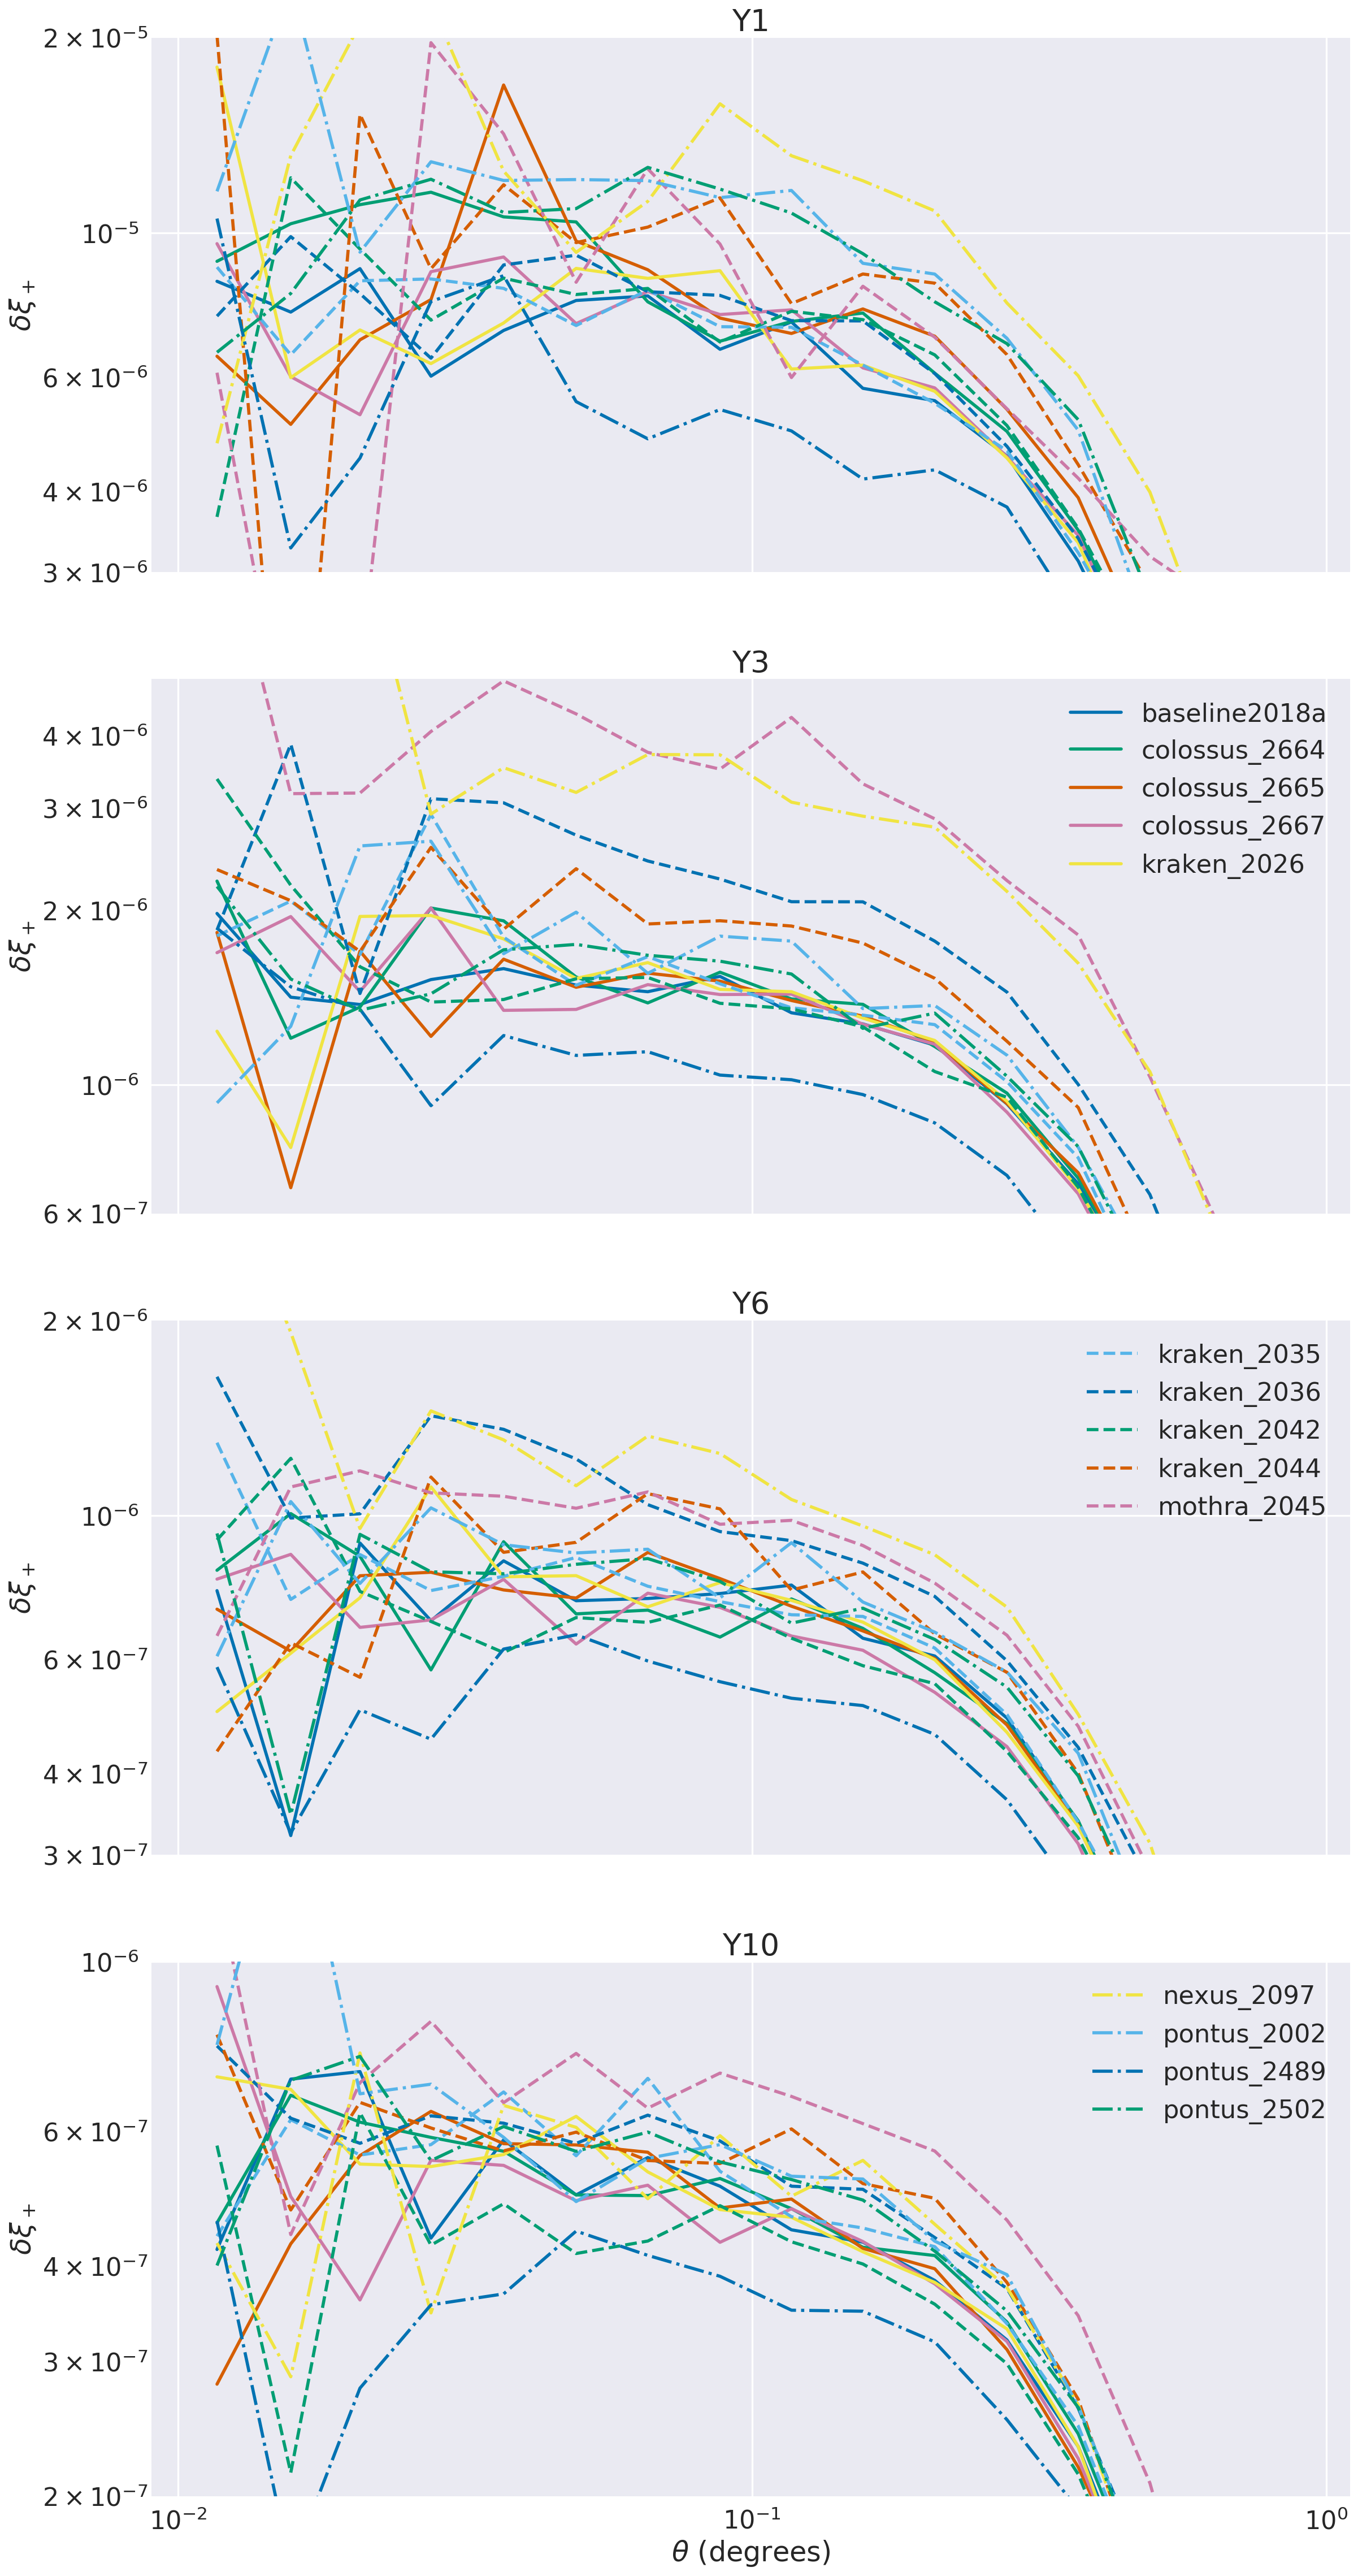
\includegraphics[width=0.72\textwidth]{figures/WLSystematicsAllYears.png}
\end{figure}




\begin{table}[ht]
\caption{A ranking of the recent observing strategies with respect to weak lensing systematics, as explained in the text, for years 1 and 10. Repeated numbers are ties. $<N>_i^{(Y10)}$ is the number of observations in $i$-band for objects on average after 10 years -- a simple metric that strongly correlates with the performance of an OpSim run, $<N>_i^{(Y10)}$ is typically higher for better-performing runs.}
\begin{tabular}{lllll}
\label{table:WLSystematicsRankings}
OpSim run & Y1 & Y10 & $<N>_i^{(Y10)}$ \\ \hline
mothra\_2045   & {\color{orange}9} & {\color{red}14}    & 134 \\
kraken\_2044   & {\color{red}11}   & {\color{red}13}    & 162 \\
nexus\_2097    & {\color{red}14}   & {\color{red}12}    & 159 \\
pontus\_2002   & {\color{red}12}   & {\color{red}11}    & 160 \\
kraken\_2036   & {\color{yellow}6} & {\color{orange}10} & 178 \\
pontus\_2502   & {\color{red} 12}  & {\color{orange}9}  & 179 \\
kraken\_2035   & {\color{green}2}  & {\color{yellow}8}  & 210 \\
colossus\_2664 & {\color{yellow}6} & {\color{yellow}7}  & 208 \\
kraken\_2026   & {\color{green}2}  & {\color{yellow}5}  & 217 \\
baseline2018a  & {\color{green}2}  & {\color{yellow}5}  & 212 \\
colossus\_2665 & {\color{orange}9} & {\color{green}3}   & 210 \\ 
colossus\_2667 & {\color{green}2}  & {\color{green}3}   & 220 \\
kraken\_2042   & {\color{orange}8} & {\color{green}2}   & 234 \\
pontus\_2489   & {\color{green}1}  & {\color{green}1}   & 306

\end{tabular}
\end{table}

There are several metrics that contain similar information to that in our analysis in MAF: the distribution of angles pointing to the center of the field of view in each observation \footnote{\url{https://github.com/LSST-nonproject/sims\_maf\_contrib/blob/5fd4ad762509cab0b4e403d84f2e65ed1ad08c06/science/static/WeakLensing\_Focal\_Angle.ipynb}} from Peter Yoachim which returns the Kolmogorov-Smirnov test's D-statistic for this distribution of angles against a uniform distribution, the distribution of coadded-depth (high values and narrow distribution is best) the distribution of airmass (low values and narrow distribution is best), the distribution of seeing values (also low values and narrow distribution is best). The reason these metrics provide similar results to our analysis is that survey uniformity is one of the crucial things that averages down WL systematics, and all these metrics are, in one way or another, a measure of uniformity.


